%%%------------------------------------------------------------------------------------------------------------
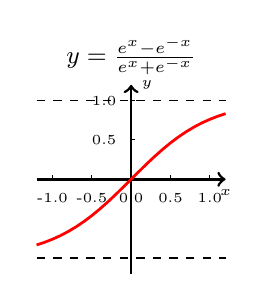
\begin{tikzpicture}
        \draw[->, line width=1pt](-1.2,0)--(1.2,0)node[left,below,font=\tiny]{$x$};
        \draw[->, line width=1pt](0,-1.2)--(0,1.2)node[right,font=\tiny]{$y$};
        \draw[dashed](-1.2,1)--(1.2,1);
        \draw[dashed](-1.2,-1)--(1.2,-1);
        \foreach \x in {-1.0,-0.5,0.0,0.5,1.0}{\draw(\x,0)--(\x,0.05)node[below,outer sep=2pt,font=\tiny]at(\x,0){\x};}
        \foreach \y in {0.5,1.0}{\draw(0,\y)--(0.05,\y)node[left,outer sep=2pt,font=\tiny]at(0,\y){\y};}
        \draw[color=red ,domain=-1.2:1.2, line width=1pt]plot(\x,{tanh(\x)});
        \node[black,anchor=south] at (0,1.2) {\small $y = \frac{e^{x}-e^{-x}}{e^{x}+e^{-x}}$};
        \end{tikzpicture}
%%%------------------------------------------------------------------------------------------------------------

